\documentclass[a4paper,11pt]{article}

\usepackage[utf8]{inputenc}
\usepackage[swedish]{babel}
\usepackage[top=1in,bottom=1in,left=1in,right=1in,headsep=.5in]{geometry}
\usepackage{hyperref}
\usepackage{graphicx}
\usepackage{pdfpages}
\usepackage{siunitx}

\usepackage{tikz}
\usetikzlibrary{shapes.geometric, shapes.misc, arrows, calc}

\usepackage{array}
\newcolumntype{L}[1]{>{\raggedright\let\newline\\\arraybackslash\hspace{0pt}}m{#1}}
\newcolumntype{C}[1]{>{\centering\let\newline\\\arraybackslash\hspace{0pt}}m{#1}}
\newcolumntype{R}[1]{>{\raggedleft\let\newline\\\arraybackslash\hspace{0pt}}m{#1}}

\usepackage[yyyymmdd,hhmmss]{datetime}
\renewcommand{\dateseparator}{-}

\usepackage{mathptmx}    %Times Roman font
\usepackage{helvet}    %Helvetica, served as a model for arial
\usepackage{anyfontsize}

\usepackage[tocgraduated]{tocstyle}
\usetocstyle{allwithdot}

\usepackage[titletoc,title]{appendix}

\usepackage[backend=bibtex,style=authoryear,maxcitenames=2,maxbibnames=9]{biblatex} %Harvard-style citations
\setlength{\bibitemsep}{\baselineskip}	%vertical space between bibliography items

\usepackage{fancyhdr}
\fancypagestyle{intro}{
    \fancyhf{}
    \fancyhead[C]{\LIPSprojekttitel}
    \fancyhead[R]{\today} 
    \fancyfoot[L]{\LIPSkursnamn \\ \LIPSdokumenttyp}
    \fancyfoot[C]{\phantom{text}\roman{page}}
    \fancyfoot[R]{\LIPSprojektgrupp \\ \LIPSgruppepost} 
    \renewcommand{\headrulewidth}{0.4pt}
    \renewcommand{\footrulewidth}{0.4pt}}
\fancypagestyle{content}{
    \fancyhf{}
    \fancyhead[C]{\LIPSprojekttitel}
    \fancyhead[R]{\today} 
    \fancyfoot[L]{\LIPSkursnamn \\ \LIPSdokumenttyp}
    \fancyfoot[C]{\phantom{text}\thepage}
    \fancyfoot[R]{\LIPSprojektgrupp \\ \LIPSgruppepost} 
    \renewcommand{\headrulewidth}{0.4pt}
    \renewcommand{\footrulewidth}{0.4pt}}

\usepackage{titlesec}
\titleformat{\section}
    {\normalfont\sffamily\Large\bfseries}
    {\thesection}{1em}{}
\titleformat{\subsection}
    {\normalfont\sffamily\large\bfseries}
    {\thesubsection}{1em}{}
\titleformat{\subsubsection}
    {\normalfont\sffamily\bfseries}
    {\thesubsubsection}{1em}{}

\newcommand{\LIPSartaltermin}{2016/HT}
\newcommand{\LIPSkursnamn}{TSEA29}
\newcommand{\LIPSprojekttitel}{Kartrobot}
\newcommand{\LIPSprojektgrupp}{Grupp 1}
\newcommand{\LIPSgruppepost}{\href{mailto:kmm_2016_grupp1@liuonline.onmicrosoft.com}{{\small kmm\_2016\_grupp1@liuonline.onmicrosoft.com}}}
\newcommand{\LIPSgrupphemsida}{}
\newcommand{\LIPSkund}{ISY, Linköpings universitet, 581\,83 Linköping}
\newcommand{\LIPSkundkontakt}{Mattias Krysander, 013-282198, matkr@isy.liu.se}
\newcommand{\LIPSkursansvarig}{Tomas Svensson, 013-281368, Tomas.Svensson@liu.se}
\newcommand{\LIPShandledare}{Olov Andersson, 013-282658, olov@isy.liu.se}
\newcommand{\LIPSdokumenttyp}{Användarhandledning}
\newcommand{\LIPSredaktor}{Silas Lenz}

\newcommand{\LIPSversion}{1.0}
\newcommand{\LIPSgranskare}{Felix Härnström}
\newcommand{\LIPSgranskatdatum}{2016-12-13}
\newcommand{\LIPSgodkannare}{}
\newcommand{\LIPSgodkantdatum}{}

\newcommand{\LIPStitelsida}{
\vspace*{200pt}
\renewcommand{\familydefault}{\sfdefault}	%Sans-serif
\normalfont
\begin{center}
{\fontsize{18}{22}\selectfont \textbf{\MakeUppercase{\LIPSdokumenttyp}}}
\end{center}
\begin{center}
{\fontsize{12}{14}\selectfont \LIPSredaktor \\[8pt] Version \LIPSversion}
\end{center}
\vspace*{220pt}
\begin{center}
{\fontsize{12}{14}\selectfont Status}
\end{center}
\begin{center}
\setlength\extrarowheight{2pt}
\begin{tabular}{| L{100pt} | L{100pt} | L{100pt} |}
\hline 
Granskad & \LIPSgranskare & \LIPSgranskatdatum \\
\hline 
Godkänd & \LIPSgodkannare & \LIPSgodkantdatum \\ 
\hline 
\end{tabular} 
\end{center}
\renewcommand{\familydefault}{\rmdefault}	%Back to serifs
\normalfont
}


\newenvironment{LIPSprojektidentitet}{%
\vspace*{200pt}
\renewcommand{\familydefault}{\sfdefault}	%Sans-serif
\normalfont
\begin{center}
{\fontsize{16}{19}\selectfont \textbf{PROJEKTIDENTITET}}
\end{center}
\renewcommand{\familydefault}{\rmdefault}	%Back to serifs
\normalfont
\begin{center}
\LIPSartaltermin, \LIPSprojektgrupp \\ Linköpings tekniska högskola, ISY
\end{center}
\renewcommand{\familydefault}{\sfdefault}	%Sans-serif
\normalfont
\vspace*{10pt}
\begin{center}
\setlength\extrarowheight{2pt}
\begin{tabular}{| L{100pt} | L{150pt} | L{150pt} |}
\hline
\textbf{Namn} & \textbf{Ansvar} & \textbf{E-post} \\
}%
{%
\hline
\end{tabular} 
\end{center}
\renewcommand{\familydefault}{\rmdefault}	%Back to serifs
\normalfont
\begin{center}
\textbf{E-postlista för hela gruppen:} \LIPSgruppepost \\
\textbf{Hemsida:} \LIPSgrupphemsida \\
\vspace*{15pt}
\textbf{Kund:} \LIPSkund \\
\textbf{Kontaktperson hos kund:} \LIPSkundkontakt \\
\vspace*{15pt}
\textbf{Kursansvarig:} \LIPSkursansvarig \\
\textbf{Handledare:} \LIPShandledare \\
\end{center}
}
\newcommand{\LIPSgruppmedlem}[3]{\hline {#1} & {#2} & \href{mailto:{#3}}{{#3}} \\}

\newenvironment{LIPSdokumenthistorik}{%
\vspace*{100pt}
\renewcommand{\familydefault}{\sfdefault}	%Sans-serif
\normalfont
\begin{center}
{\fontsize{14}{17}\selectfont \textbf{Dokumenthistorik}}
\end{center}
\begin{center}
\setlength\extrarowheight{2pt}
\begin{tabular}{| L{50pt} | L{60pt} | L{150pt} | L{60pt} | L{55pt} |}
\hline
\textbf{Version} & \textbf{Datum} & \textbf{Utförda förändringar} & \textbf{Utförda av} & \textbf{Granskad} \\
}%
{%
\hline
\end{tabular} 
\end{center}
\renewcommand{\familydefault}{\rmdefault}	%Back to serifs
\normalfont
}
\newcommand{\LIPSversionsinfo}[5]{\hline {#1} & {#2} & {#3} & {#4} & {#5} \\}

\newcounter{LIPSkravnummer}
\newcounter{LIPSunderkravnummer}[LIPSkravnummer]
\newenvironment{LIPSkravlista}{%
\renewcommand{\familydefault}{\sfdefault}	%Sans-serif
\normalfont
 \setlength\extrarowheight{2pt}
  \begin{tabular}{| L{30pt } | L{60pt} | L{250pt} | L{50pt} |}
    }%
  {%
    \hline
  \end{tabular}
\renewcommand{\familydefault}{\rmdefault}	%Back to serifs
\normalfont
}
\newcommand{\LIPSkrav}[3]{\hline\stepcounter{LIPSkravnummer}\textbf{\arabic{LIPSkravnummer}} & \textbf{{#1}} & {#2} & \textbf{{#3}} \\}

\newcommand{\LIPSkravDemo}[3]{\hline\textbf{X} & \textbf{{#1}} & {#2} & \textbf{{#3}} \\}

\newcommand{\LIPSunderkrav}[3]{\hline\stepcounter{LIPSunderkravnummer}\textbf{\arabic{LIPSkravnummer}\Alph{LIPSunderkravnummer}} & \textbf{{#1}} & {#2} & \textbf{{#3}} \\}


\newenvironment{LIPSleveranslista}{
\renewcommand{\familydefault}{\sfdefault}	%Sans-serif
\normalfont
	\setlength\extrarowheight{2pt}
	\begin{tabular}{| L{25mm} | L{25mm} | L{55mm} | L{25mm} | L{5mm} |} 
	}
	{
		\hline
	\end{tabular}
\renewcommand{\familydefault}{\rmdefault}	%Back to serifs
\normalfont
}
\newcommand{\LIPSleverans}[4]{ \hline\stepcounter{LIPSkravnummer}\textbf{Krav nr \arabic{LIPSkravnummer}}&\textbf{{#1}}&{#2}&\textbf{{#3}}&\textbf{{#4}}\\}


\newenvironment{LIPSdokumentlista}{%
	\renewcommand{\familydefault}{\sfdefault}	%Sans-serif
	\normalfont
	\setlength\extrarowheight{2pt}
	\begin{tabular}{| L{40mm} | L{13mm} | L{50mm} | L{19mm} | L{14mm} |} 
		
		\hline
		\textbf{Dokument} & \textbf{Språk} & \textbf{Syfte/Innehåll} & \textbf{Målgrupp} & \textbf{Format} \\
	}%
	{%
		\hline
	\end{tabular}
	\renewcommand{\familydefault}{\rmdefault}	%Back to serifs
	\normalfont
}
\newcommand{\LIPSdokument}[5]{\hline {#1} & {#2} & {#3} & {#4} & {#5}\\}


\begin{document}

\pagestyle{intro}
\LIPStitelsida
\clearpage
\begin{LIPSprojektidentitet}
    \LIPSgruppmedlem{Hannes Haglund}{Designansvarig mjukvara (MV)}{hanha265@student.liu.se}
    \LIPSgruppmedlem{Felix Härnström}{Projektledare (PL)}{felha423@student.liu.se}
    \LIPSgruppmedlem{Jani Jokinen}{Leveransansvarig (LEV)}{janjo273@student.liu.se}
    \LIPSgruppmedlem{Silas Lenz}{Testansvarig (TST)}{sille914@student.liu.se}
    \LIPSgruppmedlem{Daniel Månsson}{Designansvarig hårdvara (HV)}{danma344@student.liu.se}
    \LIPSgruppmedlem{Emil Norberg}{Dokumentansvarig (DOK)}{emino969@student.liu.se}
\end{LIPSprojektidentitet}

\clearpage
\renewcommand{\familydefault}{\sfdefault}	%Sans-serif
\normalfont
\tableofcontents
\renewcommand{\familydefault}{\rmdefault}	%Back to serifs
\normalfont
\clearpage
\begin{LIPSdokumenthistorik}
    \LIPSversionsinfo{1.0}{2016-12-13}{Första versionen.}{FH, SL}{FH}
\end{LIPSdokumenthistorik}
\clearpage
\setcounter{page}{1}
\pagestyle{content}

\section{Anslutning}
Vid strömpåslag kommer roboten automatiskt starta upp och ansluta till \texttt{eduroam}. Dess IP-adress kommer postas till gruppens Slack-kanal, men kan också avläsas genom att koppla in en skärm till Raspberry Pi och köra kommandot \texttt{sudo ip addr}. Detta kan sedan användas för att ansluta med PC-mjukvaran, eller via SSH med användarnamn \texttt{pi} och lösenord \texttt{mpu6050}.

\section{Uppstart}
\begin{enumerate}
    \item Det rekommenderas att starta om robotens AVR-processorer genom att trycka in den röda knappen på övre virkortet innan körning (se punkt 1 i figur \ref{fig:robot_overview}, bilaga \ref{app:picture}), för att kalibrera sensorer. Se till att roboten står stilla under kalibrering.
    
    \item Starta upp PC-mjukvaran genom ändra IP-adress i \texttt{main.py} och därefter köra \texttt{python3 main.py}. 
\end{enumerate}

\section{GUI}\label{sec:gui}
Det grafiska gränssnittet har knappar för att byta läge, samt för att stänga av programmet. I det manuella läget kan piltangenterna på tangentbordet användas för styrning. Även flera tangenter samtidigt fungerar. Till vänster visas en karta i det autonoma läget. Till höger visas sensordata och i mitten visas aktuell motorstatus samt kontrollpanelen. Se figur \ref{fig:gui} för en bild av gränssnittet.

\begin{figure}[h!]
    \centering
    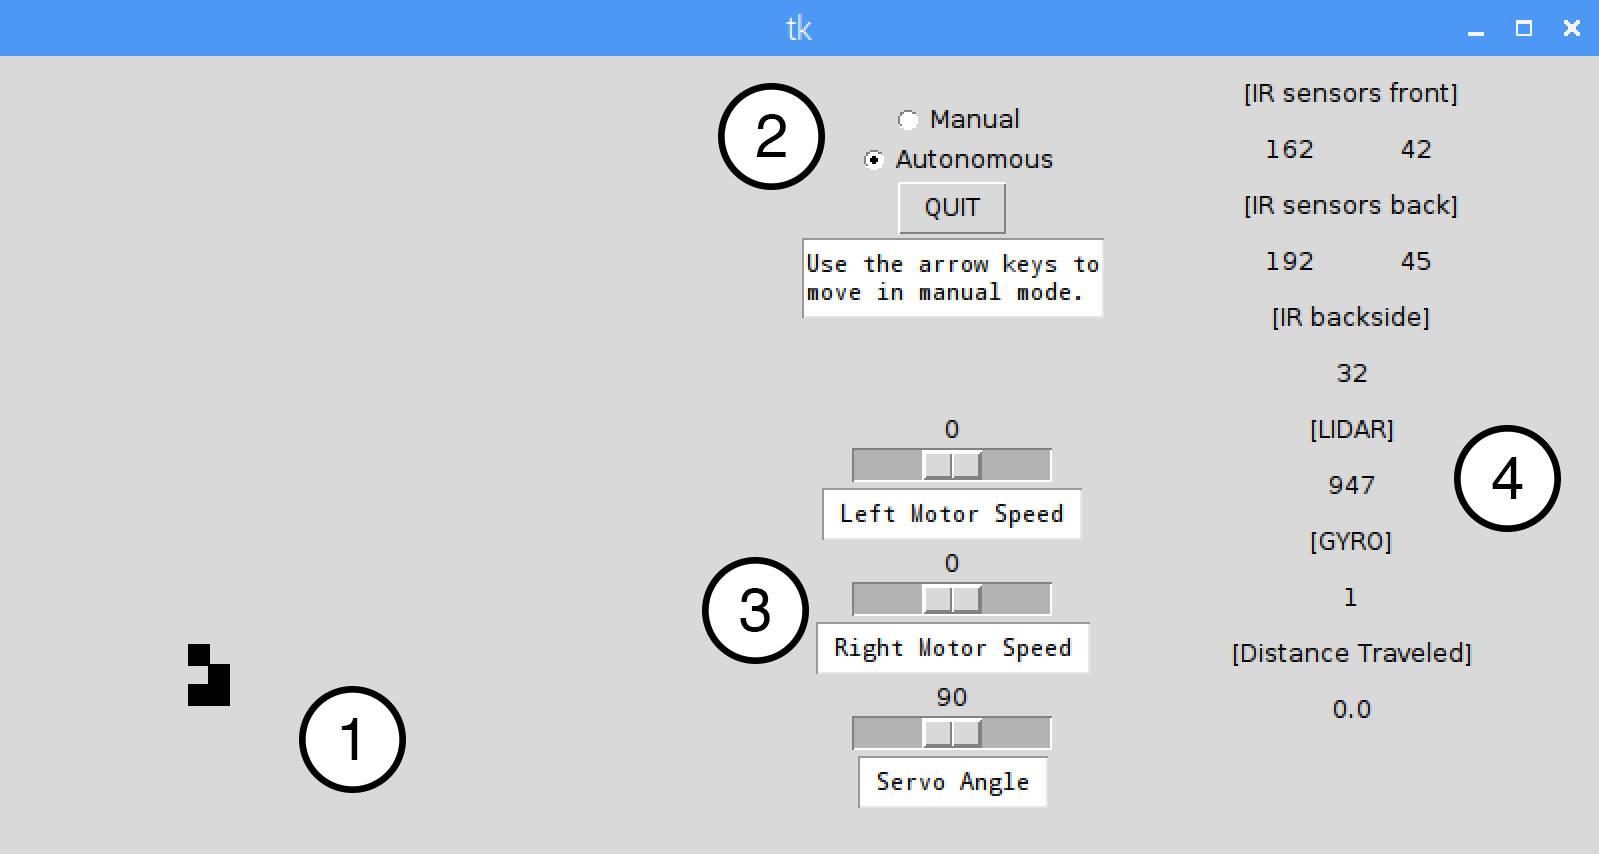
\includegraphics[scale=0.55]{gui_annotated.png}
    \caption{Det grafiska gränssnittet.}
    \label{fig:gui}
\end{figure}

Siffrorna i figur \ref{fig:gui} står för följande delar av det grafiska gränssnittet;
\begin{enumerate}
\item Hitintills utritad karta.
\item Knappar för att byta läge och stänga ner PC-mjukvaran.
\item Nuvarande motorhastighet och servoposition.
\item Nuvarande sensorvärden och avverkat avstånd.
\end{enumerate}

\section{Byta läge}
För att byta mellan autonomt och manuellt kan det grafiska gränssnittet (se kapitel \ref{sec:gui}) eller den blåa fysiska knappen på roboten användas (se punkt 3 i figur \ref{fig:robot_overview}, bilaga \ref{app:picture}).

\section{Avstängning}
För att stänga av roboten måste kommunikations- och kontrollenheten genomföra en mjuk avstängning innan strömmen bryts. För att stänga av kommunikations- och kontrollenheten trycker man ned den röda knappen på roboten (se punkt 2 i figur \ref{fig:robot_overview}, bilaga \ref{app:picture}).

\clearpage
\begin{appendices}
\section{Produktbild}\label{app:picture}
 \begin{figure}[h!]
     \centering
     \includegraphics[scale=0.15]{robot_side_annotated.png}
     \caption{Översikt över roboten.}
     \label{fig:robot_overview}
 \end{figure}
\end{appendices}

\end{document}
